%==========================================================
% Monografia de conclusao de curso apresentada ao ICMC para
% obtencao do titulo de Mestre em Ciencia de Computacao,
% novembro de 2007.
% 
% Autor
% Heitor Luis Polidoro
% 
% Orientador
% Prof. Dr. Denis Fernando Wolf
%==========================================================

\documentclass[12pt,a4paper,twoside,openright,final]{report}
\usepackage{monoproj}

\begin{document}
	
	%--------------------------------------------------------
	% Capa e Folha de Rosto
	%--------------------------------------------------------
	\title{Desenvolvimento de Rotas para Monitorar Ambientes Internos}
	\author{Heitor Luis Polidoro}
	\supervisor{Prof. Dr. Denis Fernando Wolf}
	\date{S�o Carlos / SP\\Fevereiro de 2010}
	\concarea{Rob�tica M�vel, Monitoramento, Navega��o.}
	\maketitle
	%--------------------------------------------------------

  \cleardoublepage
	\setcounter{page}{1}
	\pagenumbering{roman}
	
	%--------------------------------------------------------
	% Agradecimento
	%--------------------------------------------------------
%	%==========================================================
% Projeto de Mestrado
% 
% Agradecimento.
% 
% Autor
% Heitor Luis Polidoro
% 
% Orientador
% Prof. Dr. Denis Fernando Wolf
%==========================================================

\pagestyle{abstractst}

\chapter*{Agradecimento}
 \label{agradecimento}
 Agradeça aqui

	%--------------------------------------------------------
	% Dedicat�ria
	%--------------------------------------------------------
%	%==========================================================
% SCE=567 Projeto Supervisionado ou de Graduacao II
% 
% Dedicat�ria.
% 
% Autor
% Heitor Luis Polidoro
% 
% Orientador
% Prof. Dr. Denis Fernando Wolf
%==========================================================

\pagestyle{abstractst}

\chapter*{Dedicat�ria}
\label{dedicatoria}
Dedico o resultado deste projeto aos meus pais, Heitor e Sonia, pois sem o esfor�o e dedica��o de ambos n�o seria poss�vel eu estudar em uma universidade de renome. Exalto os esfor�os de ambos para que eu tivesse uma educa��o de qualidade e pelos exemplos de profissionalismo e educa��o, fazendo com que desta forma, me tornasse um bom cidad�o e profissional capacitado. Por toda a sua dedica��o, carinho e compreens�o, lhes sou muito grato.
	%--------------------------------------------------------
	% Resumo
	%--------------------------------------------------------
	%==========================================================
% Resumo
% 
% Autor
% Heitor Luis Polidoro
% 
% Orientador
% Prof. Dr. Denis Fernando Wolf
%==========================================================

\pagestyle{chapterst}

\chapter*{Resumo}
\label{Resumo}
A rob�tica m�vel � uma �rea de pesquisa que est� obtendo grande aten��o da comunidade cient�fica. O desenvolvimento de rob�s m�veis aut�nomos, que sejam capazes de interagir com o ambiente, aprender e de tomar decis�es corretas para que suas tarefas sejam executadas com �xito � o maior desafio em rob�tica m�vel. O desenvolvimento destes sistemas inteligentes e aut�nomos consiste em uma �rea de pesquisa multidisciplinar, considerada recente e extremamente promissora que envolve: intelig�ncia artificial, aprendizado de m�quina, estima��o estat�stica e sistemas embarcados, por exemplo. Dentro desse contexto, esse trabalho aborda o problema de navega��o e monitoramento de ambientes utilizando rob�s m�veis. Dado uma representa��o do ambiente (mapa topol�gica) e uma lista com urg�ncias de cada uma das regi�es do mapa, o rob� deve estimar qual o percurso mais eficiente para monitorar esse ambiente. Uma vez que a urg�ncia de cada regi�o n�o visitada aumenta com o tempo, o trajeto do rob� deve-se adaptar a essas altera��es. Entre as diversas aplica��es pr�ticas desse tipo de algoritmo, destaca-se o desenvolvimento de sistemas de seguran�a m�veis inteligentes. Experimentos com diferentes algoritmos em diferentes ambientes s�o apresentados.

	%--------------------------------------------------------
	
	%--------------------------------------------------------
	% Sumario e Lista de Figuras, Tabelas, Algoritmos etc.
	%--------------------------------------------------------
	\tableofcontents
	\listoffigures
%	\listoftables
	\listofalgorithms
	%--------------------------------------------------------
	
	\cleardoublepage
	\setcounter{page}{1}
	\pagenumbering{arabic}
	
	%--------------------------------------------------------
	% Corpo da Monografia
	%--------------------------------------------------------
	%==========================================================
% Capitulo 1: Introducao.
% 
% Autor
% Heitor Luis Polidoro
% 
% Orientador
% Prof. Dr. Denis Fernando Wolf
%==========================================================

\pagestyle{chapterst}

\chapter{Introdu��o}
\label{introducao}

\section{Contextualiza��o}
\label{contextualizacao}
Os rob�s s�o uma tecnologia utilizada para auxiliar ou substituir o homem em tarefas em ambientes insalubres, como fundo do mar, inc�ndios, desarmamento de bombas, �reas com contamina��o radioativa ou com gases t�xicos, em tarefas repetitivas como uma linha de produ��o industrial, em tarefas que o ser humano n�o � capaz de executar, ou tarefas sem valor intelectual.

Entre todas essas diversas aplica��es da rob�tica m�vel, pode-se citar o rob� Sojourner (Figura \subref{fig:sojourner}) da NASA, que explorou e enviou fotos e outras muitas informa��es do planeta Marte para a Terra \cite{NASA}, e o rob� desenvolvido pela universidade Camegie Mellon, chamado Groundhog, que explora minas abandonadas, que al�m do risco de desabamento, em muitos casos tamb�m cont�m gases t�xicos \cite{Thrun2004}.

Dentre as muitas defini��es de rob� podemos destacar:
\begin{itemize}
	\item Dispositivo ou m�quina que realiza fun��es normalmente associadas a seres humanos \cite{Medeiros1998};
	\item M�quinas que, al�m de serem capazes de reproduzir tarefas	e movimentos impl�citos em sua contru��o, complementam a parte mec�nica com dispositivos eletr�nicos inteligentes \cite{Medeiros1998};
	\item Um �rg�o mec�nico vers�rio equipado com atuadores e sensores sob o controle de um sistema computacional \cite{Latombe1991};
	\item Simplesmente um agente artificial e ativo cujo ambiente � o mundo f�sico \cite{Russell2003};
\end{itemize}

Inicialmente, os rob�s foram utilizados para automa��o industrial, presos em posi��es espec�ficas na linha de montagem, os bra�os rob�ticos podem mover-se a uma grande velocidade e precis�o para realizar tarefas repetitivas. Gra�as a essa precis�o sobre-humana � poss�vel a constru��o de \textit{Notebooks} e telefones port�teis. No entranto esses rob�s sofrem uma fundamental disvantagem: Falta de mobilidade. Um manipulador fixo tem alcance limitado que depende de onde foi colocado. Rob�s m�veis, entretando, s�o capazes de locomoverem-se pela f�brica \cite{Siegwart2004}. Mas com a evolu��o tecnol�gica os rob�s passaram a ser utilizados em outras �reas como: medicina de precis�o, ambientes perigosos, ambientes insalubres, na �rea de entretenimento, servi�os dom�sticos, etc. Nesse contexto surgiram as pesquisas para o desenvolvimento de rob�s m�veis aut�nomos, que sejam capazes de atuar em ambientes reais e reagir a situa��es desconhecidas de forma inteligente \cite{Thrun2002}.

A comunidade cient�fica aposta que sistemas rob�ticos estejam cada vez mais presentes em nossa vida cotidiana, o que torna esta �rea de pesquisa extremamente promissora e desafiadora. Segundo \cite{Gates2007}, estamos entrando numa nova era da computa��o, comparando os rob�s industriais com os mainframes de antigamente, e prev� que existir� um rob� em cada casa no futuro.

A rob�tica consiste em uma �rea multidisciplinar de pesquisa, envolvendo desde elementos de engenharia mec�nica, el�trica, computa��o at� �reas de humanas como psicologia e estudos do comportamentais. O que diferencia a rob�tica m�vel de outras �reas de pesquisa em rob�tica, � a sua �nfase nos problemas relacionados com locomo��o em ambientes complexos, que se modificam dinamicamente, compostos tanto por obst�culos fixos quanto por obst�culos m�veis. Para operar nesses ambientes o rob� deve ser capaz de adquirir e utilizar conhecimento sobre o ambiente, tais como: estimar posi��es dentro do ambiente (sua posi��o, de um obst�culo, de um \textit{landmark}, de uma meta, et al.), reconhecer obst�culos, e responder em tempo real �s situa��es que podem ocorrer nesses ambientes. As tarefas de perceber o ambiente, se localizar no ambiente e mover-se pelo ambiente s�o problemas fundamentais da rob�tica m�vel \cite{Heinen2002}. 

A rob�tica m�vel, al�m de ser uma �rea de grande potencial cient�fico, empresas de tecnologia est�o cada vez mais investindo em produtos. Como por exemplo o desenvolvimento de rob�s que realizam trabalhos dom�sticos autonomamente,  entre os quais o aspirador de p� Roomba da IRobot \cite{IRobot} (Figura \subref{fig:roomba}) e o rob� cortador de grama Robomow (Figura \subref{fig:robomow}) da Friendly Robotics \cite{FriendlyRobotics}. Ambos apresentam sucesso comercial. 

\begin{figure}[ht]
  \centering
	\subfigure[Sojourner]{
    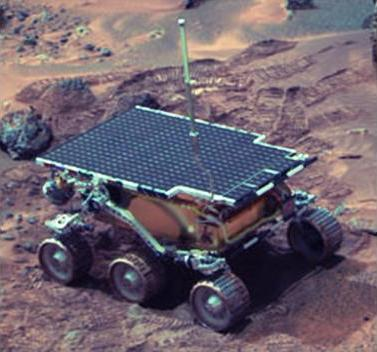
\includegraphics[width=0.4\textwidth]{../imagens/sojourner.jpg}
		\label{fig:sojourner}}	
	\subfigure[Roomba]{
	  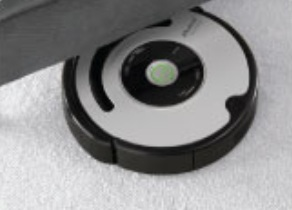
\includegraphics[width=0.4\textwidth]{../imagens/roomba.jpg}
		\label{fig:roomba}}
	\subfigure[Robomow]{
	  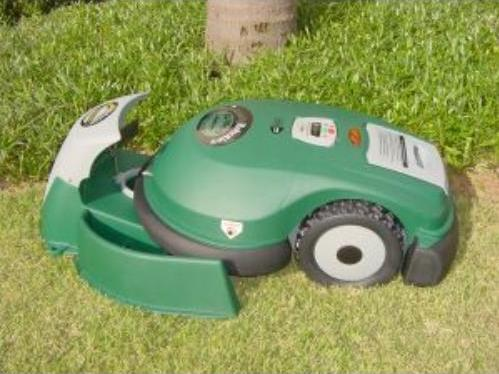
\includegraphics[width=0.4\textwidth]{../imagens/robomow.jpg}
		\label{fig:robomow}}
	\label{fig:exemplo_de_robos}
	\caption{Exemplos de rob�s.}
\end{figure}


Rob�s m�veis podem ser classificados como: homan�ides, com pernas e com rodas. Rob�s com rodas s�o mais simples de serem constru�dos e mais f�ceis de controlas, as rodas permitem uma maior praticidade de locomo��o e d�o um maior suporte est�tico ao rob� \cite{Russell2003}. A autonomia de rob�s m�veis � essencial em ambientes remotos, tais como planetas distantes, onde o tempo de comunica��o entre o rob� e seu operador n�o permite seja grande o suficiente para prejudicar deci�es em tempo real.

Normalmente, a navega��o � a principal tarefa a ser executada por um rob� m�vel. Esta consiste nos passos de localiza��o do rob� no ambiente, planejamento de um caminho entre a posi��o inicial e o destino final e a execu��o do movimento pelo caminho planejado. Esta tarefa pode ser mais, ou menos, complexa, depende do ambiente em que o rob� se encontra \cite{Pedrosa2001}

A proposta desse projeto � desenvolver uma aplica��o de rob�tica m�vel para o monitoramento de ambientes internos, onde normalmente, nesses ambientes, existem regi�es cr�ticas que possuem prioridades distintas para serem monitoradas. A prioridade (urg�ncia) da visita de cada uma dessas regi�es aumenta conforme o tempo passa e essa regi�o n�o � visitada. Ao ser visitada, a urg�ncia de uma determinada regi�o �, ent�o, zerada. Para a solu��o do problema descrito anteriormente, sup�es-se que o rob� tenha uma descri��o do ambiente em que atua (mapa). 

Na literatura, um problema semelhante que vem sendo estudando h� muitos anos � o Problema do caixeiro-viajante da classe de problemas de roteamento de n�s, onde o caixeiro deve, dado um conjunto de cidades, partir de uma cidade base, visitar as outras somente uma vez e retornar � base \cite{Arenales2007}. 

\section{Motiva��o}
\label{motivacao}
O desenvolvimento de sistemas para controlar rob�s m�veis aut�nomos tem se mostardo um grande desafio para a Intelig�ncia Artificial. Diferentes abordagens de sistema de controle para rob�s m�veis aut�nomos vem sendo utilizadas em diversar �reas de pesquisa. Existem diversas aplica��es poss�veis para rob�s m�veis. Transporte, vigil�ncia, inspe��o, limpeza, explora��o, aux�lio a deficientes f�sicos, et al. \cite{Heinen2002}.

A motiva��o deste projeto de mestrado � desenvolver um sistema de monitoramento de ambientes internos. Existem diversas aplica��es pr�ticas para esse tipo de aplica��o. Dentre elas, pode-se citar o desenvolvimento de um rob� vigia que monitora um ambiente, dando �nfase para �reas de maior import�ncia. Outro exemplo consiste em um rob� que monitora a temperatura e umidade de ambientes onde esse fator � cr�tico. Ou at� mesmo um rob� para entregar rem�dios a pacientes em um hospital.

Durante o ano de 2006 foi iniciado o projeto de mesmo prop�sito. Foram desenvolvidos algoritmos de modo imp�rico, sem base cient�fica, por�m o projeto serviu para formar uma base de conhecimento para poder, neste projeto de mestrado, aprofundar no assunto para determinar, de modo cient�fico, o algoritmo ou estrat�gia mais eficiente para o monitoramento de ambientes internos utilizando rob�s m�veis.

\section{Objetivo}
\label{objetivo}
Esse projeto tem como objetivo o desenvolvimento e compara��o entre estrat�gias e algoritmos para determinar uma seq��ncia de �reas a serem visitadas em ambientes internos com a finalidade de monitoramento desses ambientes utilizando um rob� m�vel. O problema a ser resolvido consiste na divis�o de um ambiente previamente conhecido em �reas de interesse. A cada uma dessas �reas � atribu�do um valor (peso) referente a sua import�ncia de monitoramento. A prioridade com que o rob� deve visitar determinadas �reas � calculada com base na import�ncia dessas �reas e no tempo decorrido desde a sua �ltima visita. �reas de maior import�ncia devem ser visitadas mais freq�entemente. 

As avalia��es consistem na compara��o dos algoritmos e estrat�gias. Ser�o utilizados dois crit�rios de compara��o, um crit�rio comparando a freq��ncia relativa de cada sala com sua prioridade relativa, onde o melhor resultado � aquele em que a freq��ncia relativa se aproximar mais da prioridade relativa. O segundo crit�rio � um gr�fico mostrando a progress�o da somat�ria dos graus de urg�ncia de todas as salas.

%\section{Organiza��o da Monografia}
%\label{organizacao_monografia}
%Organiza��o da monografia.

	%==========================================================
% Rob�s M�veis.
% 
% Autor
% Heitor Luis Polidoro
% 
% Orientador
% Prof. Dr. Denis Fernando Wolf
%==========================================================

\chapter{Rob�s M�veis}
\label{robos}

\section{Locomo��o}
\label{locomocao}
Rob�s m�veis precisam de mecanismos de locomo��o que os permitam moverem-se livremente pelo ambiente, mas existe uma grande variedade de meios de se locomover, andar, pular, correr, deslisar, patinar, nadar, voar, e utilizando rodas ou esteiras \cite{Siegwart2004}. A maioria dos mecanismos de locomo��o s�o inspirados na natureza, exceto os que usam rodas ou esteiras.

Rob�s com rodas s�o os mais populares por in�meras raz�es. Rob�s com rodas s�o mecanicamente simples de construir. A raz�o da carga peso/mecanismo � favor�vel. Os outros mecanismos geralmente precisam de um hardware mais complexo para carregarem a mesma carga \cite{Jones1999}. S�o mais eficientes em gasto de pot�ncia por velocidade como mostra na Figura \ref{fig:potencia_por_velocidade}. Al�m disso, como os rob�s com rodas s�o projetados para as rodas estarem em contato com o ch�o todo o tempo, o equil�brio n�o � usualmente um problema pesquisado \cite{Siegwart2004}.

\figura{imagens/grafico_potencia_por_velocidade.png}{.5}{Pot�ncia por velocidade de v�rios mecanismos de locomo��o: (a) Rastejar e deslizar. (b) Correr. (c) Pneu em ch�o suave. (d) Andar. (e) Em ferrovia. (1) Unidade de pot�ncia (Cavalos/toneladas). (2) Velocidade (milhas/hora)}{fig:potencia_por_velocidade}

Ao inv�s de se preocupar com equil�brio, as pesquisas em rob�s com rodas tendem a focar em problemas como tra��o, estabilidade, manobrabilidade e controle \cite{Siegwart2004}. 

Existem quatro classes principais de rodas, como � mostrado na Figura \ref{fig:tipos_de_rodas}. Elas diferenciam grandemente na sua cinem�tica, e portanto a escolha da classe de roda tem um grande impacto na cinem�tica do rob� m�vel. A roda padr�o e a roda castos tem um eixo prim�rio de rota��o e s�o portanto altamente direcionais. Para mover em uma dire��o diferente, a roda precisa ser direcionada primeiro ao longo do eixo vertical. A diferen�a enter essas duas rodas � que a roda padr�o consegue concluir seu direcionamento sem efeitos colaterais, como o centro de rota��o passa pelo contato com o ch�o, ao passo que a roda castor rotaciona em torno de um eixo deslocado, causando uma for�a a ser transmitida para o chassi do rob� durante o direcionamento \cite{Siegwart2004}.

\figura{imagens/tipos_de_roda.png}{.6}{Quatro tipos b�sicos de roda. (a) Roda padr�o. (b) Roda castor. (c) Roda sueca. (d) Bola ou roda esf�rica}{fig:tipos_de_rodas}

A roda sueca e a roda esf�rica s�o ambas projetos que est�o menos condicionadas pelas direcionalidade do que a convencional roda padr�o. As fun��es da roda sueca s�o o de uma roda normal, mas prov�m baixa resist�ncia em outra dire��o, alguma vezes perpendicular � dire��o convencional, como a Sueca 90, e algumas vezes em um �ngulo intermedi�rio, como a Sueca 45. Os pequenos roletes ao redor da roda s�o passivos. A vantagem principal desse modelo � que enquanto a rota��o � provida somente atrav�s de um eixo principal, a roda pode cinematicamente mover-se com pouco atrito em diferentes poss�veis trajet�rias, n�o somente para frente e para tr�s \cite{Siegwart2004}.

A roda esf�rica � uma roda omnidirecional verdadeira, muitas vezes projetado de modo que ela possa ser alimentada ativamente para girar ao londo de qualquer dire��o. Um modo para implementar a roda esf�rica � imitar o \textit{mouse} do computador, provendo ativamente rolamentos alimentados que encostam na superf�cie superior da esfera e concedem for�a rotacional \cite{Siegwart2004}.

A principal desvantagem das rodas � que elas necessitam de uma rua ou uma superf�cie relativamente plana \cite{Braunl2008}, em terrenos desiguais, elas podem ter uma performance pobre. Genericamente, se a altura do objeto foi aproximadamente o raio da roda. Uma solu��o simples seria utilizar rodas grandes o suficiente comparada com todos os poss�veis obst�culos, mas em muitos casos isso � impratic�vel \cite{Jones1999}.

\section{Sensores}
\label{sensores}
Uma das tarefas mais importantes em um sistema aut�nomo de qualquer tipo � adquirir conhecimento sobre o ambiente. Isso � feito pegando medidas usando v�rios sensores e extraindo informa��es significativas dessas medidas \cite{Siegwart2004}. Existe um vasto n�mero de sensores sendo usados em rob�tica, aplicando diferentes t�cnicas de medidas, e usando diferentes interfaces \cite{Braunl2008}. Como humanos, n�s conseguimos ver uma x�cara em cima da mesa, e sem pensar muito conseguimos pegar essa x�cara. De fato, completar a simples tarefa de beber de uma x�cara requer uma combina��o complexa de sensores, interpreta��o, cogni��o e coordena��o \cite{Jones1999}.

Alguns sensores s�o utilizados para medidas simples como a temperatura interna de rob� ou a velocidade de rota��o dos motores, mas outros mais sofisticados podem ser utilizados para adquirir informa��o sobre o ambiente ou at� para medir diretamente a posi��o global do rob� \cite{Siegwart2004}. 

Podemos classificar os sensores em dois importantes eixos funcionais: proprioceptivo/exteroceptivo e passivo/ativo \cite{Siegwart2004}.
\textbf{Proprioceptivo}, s�o os sensores que medem valores internos ao sistema, como velocidade do motor, bateria, �ngulo dos bra�os por exemplo.
\textbf{Exteroceptivo}, s�o os sensores que adquirem informa��es sobre o ambiente do rob�, como medidos de dist�ncia, intensidade de luz, amplitude do som por exemplo. Conseq�entemente as medidas de sensores exteroceptivos s�o interpretadas pelo rob�, para extrair as informa��es significantes do ambiente.
\textbf{Passivos}, s�o sensores que medem a energia do ambiente que entra no sensor. Por exemplo: sondas de temperatura, microfones e c�meras.
\textbf{Ativos}, s�o sensores que emitem energia para o ambiente, ent�o medem a rea��o do ambiente � essa energia. Sensores deste tipo t�m uma performance superior, entretanto existem alguns riscos, como a falta de energia pode afetar a caracter�stica que o sensor est� tentando medir. Sensores ativos tamb�m podem sofrer interfer�ncias de sinais que est�o fora do seu controle. Por exemplo, sinais emitidos por rob�s pr�ximos, ou sensores similares no mesmo rob�, podem influenciar no resultado das medidas. Exemplos de sensores ativos incluem od�metro, sensores ultra-s�nicos, sonares, e LASERs para medir dist�ncia \cite{Siegwart2004}.

\section{Rob� Pioneer}
\label{robo_pioneer}

O Pioneer (Figura \ref{fig:pioneer}) � o rob� dispon�vel para testes experimentais no laborat�rio, ele � um rob� m�vel �gil, vers�til e inteligente. Constru�do em um sistema cliente-servidor, ele oferece um processamento de vis�o \textit{onboard}, comunica��o \textit{ethernet}, LASER, GPS, sonar, e outras fun��es aut�nomas. E para program�-lo deve-se utilizar a biblioteca Player \cite{MobileRobots}.

\figura{imagens/pioneer.jpg}{.9}{Rob� Pioneer.}{fig:pioneer}

\section{Controle do Rob�}
\label{controle_do_robo}
O controle do rob� ser� desenvolvido utilizando-se a biblioteca Player/Stage \cite{Gerkey2003}, a qual permite que sejam realizadas simula��es antes que os algoritmos sejam testados com o rob� real. Essas simula��es s�o importantes para o aperfei�oamento dos par�metros, como dist�ncias, velocidades, etc, antes do teste no Pioneer.


\subsection{Player}
\label{player}
O Player � um servidor de rede para controlar rob�s. Executando embarcado no rob�, o Player prov� uma interface simples e clara dos sensores e atuadores do rob� sobre uma rede IP. O programa cliente ``conversa'' com o Player utilizando sockets TCP, lendo dados dos sensores, escrevendo comandos nos atuadores e configurando dispositivos em tempo de execu��o.
O servidor Player foi desenvolvido para ser independente de linguagem e de plataforma. O programa cliente pode executar em qualquer m�quina que tenha conex�o de rede com o rob�, e pode ser escrito em qualquer linguagem que suporte sockets TCP. Atualmente existem clientes dispon�veis em C++, Tcl, Java e Phyton \cite{Player}. Futuramente, o Player n�o far� suposi��es sobre como o programa de controle do rob� � estruturado, ou seja, poder� escrever desde programas multi-threads altamente concorrentes at� programas seq��ncias simples.

\subsection{Stage}
\label{stage}
O Stage � usado normalmente como um plugin para o Player, provendo uma s�rie de dispositivos virtuais para os clientes Player. Os usu�rios escrevem as rotinas e algoritmos normalmente, como clientes para um servidor Player. N�o � poss�vel para clientes distinguir a diferen�a entre os dispositivos reais do rob� e os equivalentes simulados pelo Player/Stage. Com isso clientes Player desenvolvidos usando o Stage precisar�o de pouca ou nenhuma modifica��o para trabalhar com o rob� real, e vice-versa. Em muitos casos basta somente mudar no cliente o endere�o IP de onde est� o servidor. O Stage tamb�m pode simular uma popula��o de rob�s m�veis, sensores e objetos num ambiente bidimensional (Figura \ref{fig:stage}) \cite{Player}. Nesta disserta��o ser� utilizado somente um rob� e o sensor LASER.

\figura{imagens/stage.jpg}{.5}{Simula��o com 5 rob�s, 2 objetos, LASER, sonar e blobfinder.}{fig:stage}

	%========================================================== 
% Navega��o de Rob�s M�veis.
% 
% Autor Heitor Luis Polidoro
% 
% Orientador Prof.  Dr.  Denis Fernando Wolf
%==========================================================

\chapter{Navega��o de Rob�s M�veis} 
\label{navegacao} 
Existem diversos problemas em aberto na rob�tica m�vel.  Um dos problemas ainda em aberto consistem em um rob� com a habilidade de navegar em seu ambiente \cite{Jones1999}.  A navega��o � a ci�ncia, arte, pr�tica ou tecnologia, de planejar e percorrer uma trajet�ria de um ponto de origem at� um ponto de destino. 

Em rob�tica, navega��o � a ci�ncia de direcionar o percurso de um rob� m�vel enquanto percorre o meio ambiente (terra, �gua, ou ar).  Inerente em qualquer esquema de navega��o � o desejo de alcan�ar um destino sem se perder ou colidir com alguma coisa \cite{Mckerrow1991}.  Em geral, navega��o � um processo incremental que, segundo \cite{Murphy2000}, pode ser resolvido respondendo � quatro perguntas:

\begin{itemize} 
	\item \textbf{Para onde estou indo?} Geralmente determinado por um humano ou uma miss�o; 
	\item \textbf{Qual o melhor caminho?} Esse � o problema de planejamento de trajet�ria, e � a �rea da navega��o que recebe mais aten��o; 
	\item \textbf{Por onde passei?} Enquanto o rob� explora o ambiente, pode ser parte da miss�o mapear esse ambiente; 
	\item \textbf{Onde estou?} Para seguir uma trajet�ria ou construir um mapa o rob� precisa saber onde ele est�.  
\end{itemize}

Que podem ser sumarizadas em quatro passos, segundo \cite{Goldberg1995}:

\begin{itemize} 
	\item Percep��o e modelagem do ambiente; 
	\item Localiza��o; 
	\item Planejamento e decis�o do movimento; 
	\item Execu��o do movimento; 
\end{itemize}

A rela��o entre esses passos pode ser vista na Figura \ref{fig:fluxo_navegacao} \cite{Mckerrow1991}.

\figura{imagens/fluxo_navegacao.jpg}{.4}{Hierarquia do controle de um rob� m�vel, mostrando o fluxo de informa��o.}{fig:fluxo_navegacao}

Navega��o � a inst�ncia do paradigma geral da rob�tica ``perceber - decidir - agir''.  A implementa��o da tarefa de navega��o pode ser mais ou menos complexa, depende do contexto em que a tarefe vai ser executada \cite{Goldberg1995}.

\begin{itemize} 
	\item \textbf{O ambiente:} pode ser inicialmente conhecido, parcialmente conhecido, ou completamente desconhecido, pode ser est�tico ou com objetos m�veis, et al.; 
	\item \textbf{A meta:} pode ser especificada por \textit{landmarks} ou coordenadas; 
	\item \textbf{A navega��o em si:} pode ter restri��es como: tempo, melhor caminho, et al.; 
	\item \textbf{As habilidades do rob�:} poder de computa��o, sensores e suas incertezas, tamanho do rob� e sua cinem�tica, et al.  
\end{itemize}

A solu��o para o problema de navega��o vai depender de todas essas restri��es \cite{Goldberg1995}.

A navega��o pode ser dividida em duas grandes �reas: planejamento de trajet�ria e desvio de obst�culos.  O planejamento de trajet�ria consistem em, dado uma representa��o do ambiente (total ou parcial) o rob� deve planejar uma trajet�ria que o leve do seu ponto de origem at� seu destino, atendendo a requisitos como menor caminho ou  menos curvas por exemplo.  O desvio de obst�culos � utilizado principalmente em ambientes din�micos, onde possam haver obst�culos m�veis, e sua fun��o � fazer com que o rob� chegue em seu destino de forma segura, ou seja, n�o colida com obst�culos que podem ser m�veis ou n�o, utilizando sensores geralmente de dist�ncia, como LASERs e sonares, ou at� mesmo utilizando c�meras.

\section{Planejamento de Trajet�ria} 
\label{planejamento} 
O primeiro passo para planejar uma trajet�ria � transformar um poss�vel modelo cont�nuo do ambiente em um mapa discreto compat�vel com o algoritmo de planejamento de trajet�ria escolhido.  � poss�vel identificar tr�s estrat�gias gerais de composi��o \cite{Siegwart2004}: 

\begin{itemize} 
	\item \textit{Roadmap}: identificar um conjunto de rotas nos espa�os livres; 
	\item Decomposi��o em c�lulas: discriminar entre c�lulas livres e ocupadas; 
	\item Campos potenciais: impor uma fun��o matem�tica sobre o espa�o.  
\end{itemize}

\subsection{\textit{Roadmap}} 
\label{roadmap} 
A t�cnica de \textit{roadmap} para planejamento de trajet�rias consiste em capturar a conectividade do espa�o livre do ambiente em uma rede de curvas.  Essa rede � vista como um conjunto padr�o de caminhos.  O planejamento da trajet�ria ent�o se reduz � conectar os pontos inicial e final do rob� no \textit{roadmap} e buscar neste um caminho entre esses dois pontos. Se existir um caminho ele ser� dado pela jun��o de tr�s sub caminhos: um sub caminho entre o ponto inicial at� algum ponto do \textit{roadmap}, um sub caminho do \textit{roadmap} e um sub caminho do \textit{roadmap} at� o ponto final \cite{Ottoni2000}

V�rios m�todos propostos foram baseados nessa id�ia, dentre eles: grafos de visibilidade, diagrama de Voronoi, rede de caminho livre, e silhueta.  Nesta disserta��o ser� utilizado diagrama de Voronoi. 

\paragraph{Diagrama de Voronoi} 
\label{voronoi} 
Diagrama de Voronoi � um m�todo completo de mapa de rotas que tende � maximizar a dist�ncia enter o rob� e os obst�culos no mapa.  Para cada ponto livre no mapa � calculada a dist�ncia para o obst�culo mais pr�ximo. O diagrama de Voronoi consiste nos pontos que s�o eq�idistantes de um ou mais obst�culos.  Um exemplo de diagrama de Voronoi em um mapa pode ser visto na Figura \ref{fig:exemplo_voronoi} \cite{Siegwart2004}.

\figura{imagens/exemplo_voronoi.jpg}{.4}{Exemplo de um diagrama de Voronoi.}{fig:exemplo_voronoi}

O diagrama de Voronoi tem uma fraqueza importante no caso sensores de localiza��o com alcance limitado.  Como os algoritmo maximiza a dist�ncia entre o rob� e um objeto no ambiente, qualquer sensor de curto alcance no rob� poder� falhar para perceber ao seu redor. Se o sensor de curto alcance est� sendo usado para localiza��o, ent�o o caminho designado pelo diagrama de Voronoi ser� pobre num ponto de vista para localiza��o \cite{Siegwart2004}.

Por outro lado, como por defini��o o caminho � criado baseado em um ponto eq�idistante dos obst�culos, isso garante um rota segura do rob� pelo mapa.

\paragraph{Decomposi��o em C�lulas} 
\label{decomposicao_celulas} 
Este m�todo consiste em dividir o espa�o livre do mapa em c�lulas, de forma que um caminho entre quaisquer duas c�lulas possa ser facilmente obtido. Um grafo, chamado \textit{grafo de conectividade}, representa a rela��o de adjac�ncia enter as c�lulas.  Onde os v�rtices representam as c�lulas extra�das do espa�o livre.  Somente existe uma aresta entre dois v�rtices se e somente se as c�lulas correspondentes foram adjacentes.  O resultado de um caminho � uma seq��ncia de c�lulas denominada \textit{canal}, de onde pode ser computado um caminho cont�nuo \cite{Ottoni2000}.  A Figura \ref{fig:decomposicao_celulas} demonstra um exemplo de de mapa utilizando decomposi��o em c�lulas.

\figura{imagens/decomposicao_celulas.jpg}{.5}{Exemplo de um mapa com decomposi��o em c�lulas.}{fig:decomposicao_celulas}

\paragraph{Campos Potenciais} 
\label{campos_potenciais}
Neste m�todo o espa�o livre � discretizado em uma fina grade, a cada posi��o � associado uma fun��o, com a qual pode-se fazer uma analogia a um campo potencial.  Como o tamanho da grade � grande, pois ela � fina, s�o utilizados m�todos heur�sticos para encontrar um caminho. A analogia que o m�todo sugere � que o rob� seja uma part�cula movendo-se sob a influ�ncia de um campo potencial gerado pelos obst�culos e pelo seu ponto de destino. O ponto de destino gera um campo potencial que atrai o rob�, enquanto os obst�culos geram um campo que repele o rob�. O caminho final � dado pela for�a resultante desses campos potenciais. 

Um exemplo de campos potenciais � mostrado na Figura \ref{fig:campos_potenciais}.  O campo potencial atrativo (b) � um parabol�ide com ponto de m�nimo localizado na posi��o do objetivo.  O campo potencial repulsivo (c) � diferente de zero somente a partir de uma determinada dist�ncia dos obst�culos. O caminho (e) � constru�do pela dire��o oposta a do gradiente do potencial resultante (d). Em (f) temos uma matriz de orienta��es do vetor gradiente, que s�o as orienta��es das for�as induzidas pelo campo potencial \cite{Ottoni2000}.

\figura{imagens/campos_potenciais.jpg}{.5}{Exemplo de um mapa com campos potenciais.}{fig:campos_potenciais}

\section{Desvio de Obst�culos} 
\label{desvio} 
Recentemente, muitas pesquisas voltaram sua aten��o para o problema de desvio de obst�culos.  Entretanto, existe alguns m�todos cl�ssicos de desvio de obst�culos que dever ser citados \cite{Borenstein1991}: Detec��o de borda, \textit{certainty grid}, campos potenciais, campo de for�a virtual e vector field histogram. 

Detec��o de borda, � um m�todo bem popular que extrai as bordas verticais do objeto, e guia o rob� ao redor dessas bordas. 

\textit{Certainty grid} � um m�todo de representa��o probabil�stico de obst�culos que modela o mundo em uma grade, onde a �rea de trabalho do rob� � modelada em um arranjo de quadrados em 2D, chamada c�lulas.  Cada c�lula tem um valor de certeza que indica o grau de confian�a de que algum objeto est� na �rea dessa c�lula. 

O m�todo de campos potenciais funciona tanto para planejamento de trajet�ria quanto para desvio de obst�culos, para isso basta calcular a for�a potencial resultante em tempo de execu��o, com isso o rob� poder� desviar de obst�culos m�veis

O campo de for�a virtual (do ingl�s \textit{Virtual Force Field} - VFF) � um m�todo para ve�culos que necessitam de uma resposta mais r�pida para fazer curvas. � um m�todo baseado na \textit{certainty grid}, onde uma grade de histograma cartesiano 2D � usado para representar a probabilidade de cada c�lula conter um obst�culo, depois a id�ia de campos potenciais � aplicada ao histograma.

E por fim o m�todo de \textit{vector field histogram} - VFH, que cria um mapa de \textit{certainty grid} local, e ao inv�s de utilizar um histograma cartesiano 2D, utiliza um histograma polar ($\alpha-P$), onde $\alpha$ � o �ngulo do sensor e $P$ � a probabilidade de haver um obst�culo nessa dire��o. O VFH � explicado melhor a seguir.

Foi implementado o m�todo de campos potencias, mas ap�s alguns testes verificou-se que o m�todo VFH j� implementado no Player, � mais r�pido e mais eficiente.

\subsection{\textit{Vector Field Histogram}}
\label{VFH}
Analisando melhor o m�todo VFF percebemos um problema: redu��o dr�stica excessiva dos dados quando for�as de repuls�o individuais do histograma da grade de c�lulas s�o somadas para calcular o vetor resultante. Centenas de pontos de dados s�o reduzidos em um passo para dire��o e magnitude. Conseq�entemente, informa��es detalhadas sobre a distribui��o local do obst�culo � perdida. Para remedias essa situa��o, foi desenvolvido um novo m�todo chamado \textit{Vector Field Histogram} - VFH. O M�todo VFH utiliza dois est�gios de redu��o de dados \cite{Borenstein1991}.

Existem tr�s n�veis de representa��o de dados \cite{Borenstein1991}:

\begin{itemize}
	\item O n�vel mais alto cont�m uma descri��o detalhada do ambiente do rob�;
	\item No n�vel intermedi�rio � armazenado um histograma polar unidimensional sobre a localiza��o moment�nea do rob�;
	\item O n�vel mais baixo � a sa�da do algoritmo VFH, valores de refer�ncia para o controle de movimento do rob�
\end{itemize}

No primeiro est�gio da redu��o de dados � mapeado a grade de histograma do ambiente (Figura \ref{fig:histogram_grid})em um histograma polar (Figura \ref{fig:polar_histogram}). E no segundo est�gio computa a dire��o $\theta$ para onde o rob� deve virar.

\figura{imagens/histogram_grid.png}{.3}{(a) Exemplo de um mapa. (b) Grade de histograma correspondente.}{fig:histogram_grid}

\figura{imagens/polar_histogram.png}{.3}{(a) Densidade polar de obst�culo em um histograma polar relativo � posi��o do rob� em $O$ (Figura \ref{fig:histogram_grid}(b)). (b) O mesmo histograma polar de (a) mostrado em forma polar e por cima da grade de histograma da Figura \ref{fig:histogram_grid}(b).}{fig:polar_histogram}


\section{Representa��o do Mapa}
\label{mapa}
Representar o ambiente onde o rob� se encontra � importante pois, decis�es baseadas na representa��o do ambiente pode ter impacto nas escolhas dispon�veis para a representa��o da posi��o do rob�. Muitas vezes a fidelidade da representa��o da posi��o � limitada pela fidelidade do mapa \cite{Siegwart2004}.

Segundo \cite{Siegwart2004}, tr�s rela��es fundamentais tem de ser entendidas quando se escolha uma representa��o particular de mapa:
\begin{itemize}
	\item A precis�o do mapa precisa ser compat�vel com a precis�o da necessidade do rob� para atingir seus objetivos;
	\item A precis�o do mapa e o tipo de dados dos recursos representados precisam ser compat�veis com a precis�o e os tipo de dados retornados pelos sensores do rob�;
	\item A complexidade da representa��o do mapa tem impacto direto com a complexidade computacional.	
\end{itemize}

Existem v�rias maneira de representar um mapa: Decomposi��o por c�lula, decomposi��o fixa, decomposi��o adaptada (com varia��o de c�lula), \textit{occupancy grid} e representa��o topol�gica, et al. \cite{Siegwart2004}.


	%==========================================================
% Grafos e aplica��es.
% 
% Autor
% Heitor Luis Polidoro
% 
% Orientador
% Prof. Dr. Denis Fernando Wolf
%==========================================================
\chapter{Grafos e Aplica��es}
\label{grafos_aplicacoes}
Grafos e mapas topol�gicos, s�o muito utilizados na literatura para navega��o de rob�s m�veis, como podemos ver em \cite{Adorno2005,Scatena2004,Thrun1996,Thrun1998,Thrun1998a,Neto2003}. Como o problema proposto (se��o \ref{proposta}) diz respeito � busca de trajet�ria em um mapa topol�gico (grafo) uma das solu��es se torna uma varia��o do problema do caixeiro viajante que trata, basicamente de encontrar o menor ciclo hamiltoniano em um grafo.

As se��es seguintes cont�m uma explica��o sobre grafos, mapas topol�gicos e o problema do caixeiro viajante.

\section{Grafos}
\label{grafos}
Muitas aplica��es em computa��o necessitam considerar um conjunto de conex�es entre objetos. Os relacionamentos dessas conex�es podem ser utilizados para responder quest�es como: Existe caminho de um objeto a outro? Quantos objetos podem ser alcan�ados a partir de um determinado objeto? Qual a menor dist�ncia entre dois objetos? Existe um tipo abstrato de dados chamado grafo que � usado para modelar essas situa��es \cite{Ziviani2004}.

Um grafo � constitu�do de um conjunto de v�rtices e um conjunto de arestas que conectam pares de v�rtices. Um v�rtice � um objeto que pode conter nomes e outros atributos. Os grafos podem ser direcionados ou n�o direcionados. Um grafo direcionado $G$ � um par $(V, A)$, em que $V$ � um conjunto finito de v�rtices e $A$ � um conjunto de arestas com uma rela��o bin�ria. A Figura \ref{fig:exemplo_de_grafos}\subref{fig:grafo_dir} mostra um grafo direcionado com o conjunto de v�rtices $V = {0, 1, 2, 3, 4, 5}$ e de arestas $A = {(0, 1), (0, 3), (1, 2), (1, 3), (2, 2), (2, 3), (3, 0), (5, 4)}$. Em um grafo n�o direcionado as arestas $(u, v)$ e $(v, u)$ s�o consideradas as mesmas. A Figura \ref{fig:exemplo_de_grafos}\subref{fig:grafo_ndir} mostra um grafo n�o direcionado com o conjuntos de v�rtices $V = {0, 1, 2, 3, 4, 5}$ e de arestas $A = {(0, 1), (0, 2), (1, 2), (4, 5)}$. Em grafos direcionados podem existir arestas de um v�rtice para ele mesmo, chamadas de \textit{self-loops}, como a aresta $(2, 2)$ no grafo direcionado da Figura \ref{fig:exemplo_de_grafos}\subref{fig:grafo_dir} \cite{Ziviani2004}.

\begin{figure}[ht]
	\centering
	\subfigure[Grafo direcionado]{
		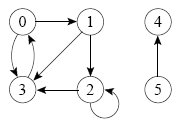
\includegraphics[width=0.2\textwidth]{imagens/grafo_direcionado.jpg}
		\label{fig:grafo_dir}}
	\subfigure[Grafo n�o direcionado]{
		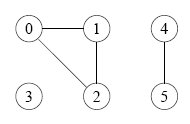
\includegraphics[width=0.2\textwidth]{imagens/grafo_nao_direcionado.jpg}
		\label{fig:grafo_ndir}}
	\caption{Exemplo de grafos\cite{Ziviani2004}}
	\label{fig:exemplo_de_grafos}
\end{figure}

Em um grafo direcionado, a aresta $(u, v)$ sai do v�rtice $u$ e entra no v�rtice $v$. Se $(u, v)$ � uma aresta do grafo $G = (V, A)$, ent�o o v�rtice $v$ � adjacente ao v�rtice $u$. Quando o grafo n�o � direcionado, a rela��o de adjac�ncia � sim�trica \cite{Ziviani2004}.

Em um grafo, um caminho $(v_0, v_1, \cdots, v_k)$ forma um clico se $v_0 = v_k$ e o caminho cont�m pelo menos uma aresta. O ciclo � simples se os v�rtices $v_1, v_2, \cdots, v_k$ s�o distintos. O \textit{self-loop} � um ciclo de tamanho 1. Na Figura \ref{fig:exemplo_de_grafos}\subref{fig:grafo_dir}, o caminho $(0, 1, 2, 3, 0)$ forma um ciclo. Dois caminhos $(v_0, v_1, \cdots, v_k)$ e $(v'_0, v'_1, \cdots, v'_k)$ formam o mesmo ciclo se existir um inteiro $j$ tal que $v'_i = v_{(j+i) mod k}$ para $i = 0, 1, \cdots, k - 1$. Na Figura \ref{fig:exemplo_de_grafos}\subref{fig:grafo_dir}, o caminho $(0, 1, 3, 0)$ forma o mesmo ciclo que os caminhos $(1, 3, 0, 1)$ e $(3, 0, 1, 3)$. Um grafo sem ciclos � um grafo ac�clico \cite{Ziviani2004}.

Um grafo $G$ � definido como \textit{Hamiltoniano} se possui um ciclo contendo todos os v�rtices de $G$. Esse nome foi dado pois, em 1856, Willian Rowan Hamilton inventou um jogo matem�tico que consistia em um dodecaedro no qual cada um dos vinte v�rtices recebeu o nome de uma cidade. O objetivo do jogo era viajar pelas arestas do dodecaedro, visitando cada cidade exatamente uma vez e retornando para o ponto inicial \cite{Beineke1978}. A Figura \ref{fig:dodecaedro_de_hamilton} mostra uma solu��o para o jogo.

\figura{imagens/dodecaedro_de_hamilton.jpg}{.5}{Dodecaedro de Hamilton.\cite{Beineke1978}}{fig:dodecaedro_de_hamilton}

Defini��es segundo \cite{Gondran1984}:

\begin{itemize}
	\item Um caminho passando somente uma vez em cada v�rtice de $G$ � chamado Caminho Hamiltoniano e tem comprimento de $N - 1$
	\item Um ciclo Hamiltoniano � um ciclo que passa somente uma vez em cada v�rtice de $G$ e tem comprimento $N$.
\end{itemize}

Um grafo n�o direcionado � conectado se cada par de v�rtices est� conectado por um caminho. Um grafo direcionado � fortemente conectado se cada dois v�rtices quaisquer s�o alcan��veis a partir um do outro. Um grafo ponderado possui pesos associados �s suas arestas. Esses pesos podem representar, por exemplo, custos ou dist�ncias. Um grafo completo � um grafo no qual todos os pares de v�rtices s�o adjacentes \cite{Ziviani2004}.

\section{Busca do Menor Caminho}
\label{busca_do_menor_caminho}
%
\subsection{Algoritmo de Dijkstra}
\label{algoritmo_de_dijkstra}
Existem diversos algoritmos para buscas em grafo na literatura \cite{Cormen2001}. Neste trabalho foi utilizado o algoritmo de Dijkstra. O algoritmo de Dijkstra utiliza a t�cnica do relaxamento, que nada mais � que verificar se � poss�vel melhorar o caminho obtido at� o momento passando por um v�rtice diferente. O algoritmo de Dijkstra apresenta uma solu��o $O([m + n] � log(n))$ para a determina��o do menor caminho \cite{Dudek2000}. E � composto por tr�s passos.

\begin{itemize}
	\item Passo 1: Iniciar os valores:

\begin{algorithmic}
	\FORALL {$v \in V[G]$} 
	\STATE$	d[v] \gets \infty$
	\STATE$ \pi[v] \gets  nulo$
	\ENDFOR
	\STATE	$d[s] \gets 0$
\end{algorithmic}

	$V[G]$ � o conjunto de v�rtices $v$ que forma o grafo $G$.
	$d[v]$ � o vetor de dist�ncias do v�rtice $s$ at� cada v�rtice $v$.
	$\pi[v]$ identifica o v�rtice de onde se origina uma conex�o at� $v$ de maneira a formar um caminho m�nimo.

	\item Passo 2: Temos que usar dois conjuntos: $S$, que representa todos os v�rtices $v$ onde $d[v]$ j� cont�m o custo do menor caminho e $Q$ que cont�m os v�rtices restantes.

	\item Passo 3: Realizamos uma s�rie de relaxamentos das arestas:
\begin{algorithmic}
	\WHILE {$Q \neq \emptyset $}
		\STATE$u \gets$ \texttt{extraia-m�n($Q$)}
		\STATE $S \gets S \cup {u}$
		\FORALL{$v$ adjacente a $u$}
			\STATE se $d[v] > d[u] + w(u, v)$ ent�o 
			\STATE $d[v] \gets d[u] + w(u, v)$
			\STATE $\pi[v] \gets u$
		\ENDFOR
	\ENDWHILE
\end{algorithmic}
		$w(u, v)$ � o peso da aresta que vai de $u$ a $v$.
		$u$ e $v$ s�o v�rtices quaisquer e $s$ � o v�rtice inicial.
		\texttt{extraia-m�n($Q$)}, retorna o menor elemento.
		
\end{itemize}

\section{Caixeiro-Viajante}
\label{caixeiro}

O problema do caixeiro-viajante envolve um conjunto de cidades e � da classe de problemas de roteamento de n�s, onde um caixeiro sai de uma cidade base, visita todas as cidades somente uma vez, e retorna � cidade base, otimizando um ou mais objetivos. Problemas de caixeiro-viajante s�o definidos em grafos orientados ou n�o orientados \cite{Arenales2007}

A defini��o do problema do caixeiro-viajante �: Considere um grafo n�o orientado $G = (N, E)$, em que o conjunto $N$ consistem em $n$ cidades e $E$ representa o conjunto de arestas entra essas cidades. Supondo que $G$ � um grafo completo, isto �, para qualquer par de cidades $i, j \in \mathbb{N}, i \neq j$, existe uma aresta $(i, j)$. A dist�ncia entre as cidades $i$, e $j$ � $c_{ij}$, e quando $c_{ij} = c_{ji}$, o problema � dito sim�trico. Um caixeiro deve visitar $n$ cidades, passando por cada cidade somente uma vez, e retornar � cidade de partida. Esse percurso � denominado ciclo Hamiltoniano do grafo $G$, e o problema consiste em determinar o ciclo Hamiltoniano, ou rota, de dist�ncia m�nima. Devido � sua aplica��o em diversas �reas, este � um dos problemas combinat�rios mais pesquisados \cite{Arenales2007}.

Defina as vari�veis

\begin{center}
$
x_{ij}=\left\{ \begin{array}{l}
			1  \mbox{ se o caixeiro vai diretamente da cidade $i$ � cidade $j$}, i \neq j \\
			0  \mbox{ se o caixeiro n�o vai da cidade $i$ � cidade $j$}, i \neq j
		\end{array}\right.
$
\end{center}

E considere o seguinte modelo:

\begin{equation}
	\mbox{min}\sum_{i=1}^n \sum_{j > i}c_{ij}x_{ij} 
	\label{eq:cv-func_obj}
\end{equation}

\begin{equation}
	\sum_{j < i} x_{ji} + \sum_{j > i} x_{ij} = 2, i = 1, \cdots, n
	\label{eq:cv-restr1}
\end{equation}

\begin{equation}
	x \in B^{n(n-1)/2}
	\label{eq:cv-restr2}
\end{equation}

A fun��o objetivo (\ref{eq:cv-func_obj}) expressa a minimiza��o da dist�ncia total da rota, e a restri��e (\ref{eq:cv-restr1}) imp�e que cada cidade tenha somente uma cidade sucessora imediata e uma cidade predecessora imediata, ou seja, � visitada uma �nica vez. Uma solu��o para o modelo anterior pode gerar sub-rotas desconexas (Figura \ref{fig:sub-rotas}) \cite{Arenales2007}.

\figura{imagens/sub-rotas.jpg}{.4}{Exemplo de poss�veis sub-rotas.\cite{Arenales2007}}{fig:sub-rotas}

Seja $S$ uma sub-rota, por exemplo, $S = {1. 2. 3. 4}$ na Figura \ref{fig:sub-rotas}. A elimina��o de sub-rotas pode ser obtida atrav�s da restri��o
\begin{equation}
	\sum_{i \in S} \sum_{i \ in S \\ j > i} \leq |S| - 1, S \subset \mathbb{N}, 3 \leq |S| \leq \left\lfloor \frac{n}{2} \right\rfloor
	\label{eq:cv-el_sub-rotas1}
\end{equation}
que garante que, para cada conjunto $S$, existem no m�nimo duas arestas que entram e/ou saem de $S$, ou seja, existem no m�nimo duas arestas entre cidades de $S$ e cidades fora de $S$. A cardinalidade de $S$ � no m�nimo 3 (pois ciclo em um grafo n�o orientado tem pelo menos 3 v�rtices) e no m�ximo $\left\lfloor\frac{n}{2}\right\rfloor$, pois ao se eliminar ciclos com $k$ v�rtices, eliminamos ciclos com $n - k$ v�rtices. A sub-rota $S = {1, 2, 3, 4}$ � eliminada.
\begin{center}
	$x_{15} + x_{16} + x_{17} + x_{25} + x_{26} + x_{27} + x_{35} + x_{36} + x_{37} + x_{45} + x_{46} + x_{47} \geq 2$
\end{center}

Uma forma alternativa de eliminar sub-rotas � com a seguinte restri��o
\begin{equation}
	\sum_{i \in S} \sum_{i \ in S \\ j > i} \leq |S| - 1, S \subset \mathbb{N}, 3 \leq |S| \leq \left\lfloor \frac{n}{2} \right\rfloor
	\label{eq:cv-el_sub-rotas2}
\end{equation}CONFERIR ESSA FORMULA EM \cite{Arenales2007}
que corresponde a eliminar uma aresta da sub-rota. A sub-rota $S = {1, 2, 3, 4}$ � eliminada.
\begin{center}
	$x_{12} + x_{23} + x_{34} + x_{14} \leq 3$
\end{center}

Como o n�mero de subconjuntos distintos de um conjunto de cardinalidade $k$ � $2^k$, as restri��es \ref{eq:cv-el_sub-rotas1} e \ref{eq:cv-el_sub-rotas2} t�m cardinalidade da ordem de $2^k$, $k \geq 6$, ou seja, o crescimento � exponencial em fun��o do n�mero de cidades. Para $k \leq 5$, somente a restri��o \ref{eq:cv-restr1} elimina sub-rotas \cite{Arenales2007}.

\section{Considera��es}
\label{consideracoes_grafo}

Como o mapa que � utilizado no projeto � um mapa baseado em grafo (mapa topol�gico), � poss�vel utilizar algumas teorias de grafos presentes na literatura como base para se achar uma solu��o para o problema. Assim como foi utilizado o algoritmo de Dijkstra nas buscas de menor caminho para o rob� fazer a menos trajet�ria de um v�rtice a outro, e a fundamenta��o matem�tica da teoria do caixeiro-viajante que foi utilizada como base para se achar uma solu��o \textit{offline}.

COLOCAR UMA SE��O DE CONSIDERA��ES PARA CONECTAR ESSE CAP�TULO AO TRABALHO.
COMENTAR QUE ESSA TEORIA FOI USADA COMO BASA PARA ACHAR A SOLU��O. FEITO?

	%==========================================================
% Resultados Obtidos.
% 
% Autor
% Heitor Luis Polidoro
% 
% Orientador
% Prof. Dr. Denis Fernando Wolf
%==========================================================

\chapter{Resultados Obtidos}
\label{resultados}

\section{Objetivo}
\label{objetivo}
Essa disserta��o tem como objetivo o desenvolvimento de uma estrat�gia eficiente para determinar uma seq��ncia de �reas a serem visitadas em ambientes internos com a finalidade de monitoramento desses ambientes utilizando um rob� m�vel. O problema a ser resolvido consiste na divis�o de um ambiente previamente conhecido em �reas de interesse (exemplo na Figura \ref{fig:mapa_museu}). A cada uma dessas �reas � atribu�do um valor (peso) referente a sua import�ncia de monitoramento (exemplo na Tabela \ref{tab:prioridade_museu}). A prioridade com que o rob� deve visitar determinadas �reas � calculada com base na import�ncia dessas �reas e no tempo decorrido desde a sua �ltima visita. �reas de maior import�ncia devem ser visitadas mais freq�entemente. 

\figura{imagens/MUSEU_DO_HOMEM_SERGIPANO.jpg}{8}{Exemplo de mapa: Museu do homem sergipano e suas divis�es}{fig:mapa_museu}

\begin{table}\begin{center}
	\begin{tabular}
		{|c|c|}
		\hline
		Sala & Prioridade \\
		\hline
		a& 5 \\
		b& 5 \\
		c& 2 \\
		d& 1 \\
		e& 3 \\
		f& 2 \\
		g& 1 \\
		h& 2 \\
		i& 2 \\
		j& 4 \\
		k& 4 \\
		l& 4 \\
		1& 2 \\
		2& 3 \\
		3& 3 \\
		4& 5 \\
		5& 5 \\
		6& 5 \\
		7& 4 \\
		8& 4 \\
		9& 3 \\
		\hline
	\end{tabular}
\end{center}
\caption{Exemplo de prioridades}
\label{tab:prioridade_museu}
\end{table}

\subsection{Crit�rios de Avalia��o}
\label{criterios}
Os algoritmos e estrat�gias ser�o ent�o testados e avaliados. As avalia��es consistem na compara��o dos algoritmos e estrat�gias. Ser�o utilizados dois crit�rios de compara��o, um crit�rio comparando a freq��ncia relativa de cada sala com sua prioridade relativa, onde o melhor resultado � aquele em que a freq��ncia relativa se aproximar mais da prioridade relativa, pois se uma sala (a) possui uma prioridade com valor duas vezes maior que uma sala (b) (Salas f e 7 na Figura \ref{tab:prioridade_museu} por exemplo), a sala (a) deve ser visitada com o dobro de freq��ncia do que a sala (b). Isto indica que o algoritmo ou estrat�gia se manteve fiel � defini��o do problema: \textit{ �reas de maior import�ncia devem ser visitadas mais freq�entemente.}.

O segundo crit�rio � um gr�fico mostrando a progress�o da somat�ria dos graus de urg�ncia de todas as salas $(\sum_{i=0}^n U_i)$ , no qual o melhor resultado consiste em manter o menor valor da somat�ria dos graus de urg�ncia. Mostrando que o algoritmo ou estrat�gia visitou as salas com maior efici�ncia. O grau de urg�ncia $U$ � calculado multiplicando-se a prioridade da sala $P$ pelo tempo decorrido desde a �ltima visita $t$. A casa visita o $t$ � zerado $(U_i = P_i \times t_i)$.

\section{Metodologia}
\label{metodologia}

Cada ambiente tem um mapa topol�gico que ser� gerado utilizando o diagrama de Voronoi. O rob� ent�o, deve utilizar deste mapa para se locomover de uma sala para outra no ambiente. Para os algoritmos e estrat�gias determinarem a seq��ncia de salas � visitar, � considerado um grafo completo com todas as salas, pois para determinar o melhor caminho entre uma sala e outra ser� utilizado o algoritmo de Dijkstra no mapa topol�gico.

Como um dos crit�rios de avalia��o est� relacionado ao tempo que o rob� fica sem visitar as salas � poss�vel deduzir que a solu��o seja um ciclo.

\pagebreak

Considere:
\begin{itemize}
	\item Um ambiente com $S$ salas;
	\item Um ciclo hamiltoniano $C$ qualquer;
	\item $C_i$ � a i-�sima sala visitada no ciclo;
	\item Uma velocidade constante do rob� (tanto linear quanto angular);
	\item $\Delta t_i$ o tempo para sair da sala $i$ e chegar na sala $i+1$.
\end{itemize}

Como o tempo de viagem de uma sala � outra � constante todos os $\Delta t_i$ s�o constantes, portanto o tempo total do ciclo $T$ � constante $(\sum_{i=1}^S \Delta t_i = cte)$. Se o tempo do ciclo � constante, o tempo que o rob� demora para revisitar cada sala � constante igual a $T$. Mas isso n�o � interessante para solu��o do problema pois o grau de urg�ncia de cada sala � diferente, ent�o se uma sala tem uma prioridade muito alta, seu grau de urg�ncia vai ser muito alto at� o rob� revisit�-la. 

Para resolver esse problema, basta fazer com que o rob� revisite essa(s) sala(s) mais de uma vez no ciclo. Ent�o supondo um ciclo de tamanho $n$ sendo $n \geq S$ o tempo total do ciclo continua constante $(\sum_{i=1}^n \Delta t_i = cte)$. Portanto a solu��o do problema consiste em encontrar esse ciclo.

MENCIONAR AS DUAS SOLU��ES, OFFLINE E REAL TIME.
EXPLICAR QUE A OFFLINE � DIVIDIDA EM 2: GERADOR E AVALIADOR


\section{Avaliador}
\label{avaliador}

O programa chamado \texttt{avaliador} � utilizado para avaliar os candidatos a seq��ncia de salas �tima do mapa analisado gerado pelo programa \texttt{gerador} \ref{gerador} e retorna para o \texttt{gerador} um valor num�rico, baseado nesse valor o \texttt{gerador} ir� guardar a seq��ncia como poss�vel �tima, descartar ou continuar utilizando essa seq��ncia para gerar novas seq��ncia. Maiores detalhes na sess�o \ref{gerador}.

\subsection{Funcionamento}

O \texttt{avaliador} recebe tr�s par�metros como entrada:
\begin{itemize}
	\item O nome do mapa onde o caminho ser� avaliado;
	\item Um vetor de v�rtices, representando a seq��ncia de salas a ser avaliada;
	\item Um valor opcional de limite para a avalia��o.
\end{itemize}

Com esses par�metros o \texttt{avaliador} inicia a simula��o do rob� navegando pelo mapa. A velocidade linear, que determina a velocidade com que o rob� anda para frente ou para tr�s, � definida pela constante \texttt{SIMULACAO\_VEL} como 1 m/s. E a velocidade angular, que determina a velocidade com que o rob� vira, � definida pela constante \texttt{SIMULACAO\_ROT} como 0.5 rad/s. Ambas constantes est�o no arquivo \texttt{robo.h}. O tempo que o rob� demora para visitar uma sala � definido pela constante \texttt{VISITAR\_SALA} como 5 s no arquivo \texttt{salas.h}.

Durante a simula��o, a cada visita de sala o \texttt{avaliador} mede o Grau de Urg�ncia Total e salva o maior valor, esse valor vai ser a avalia��o do caminho neste mapa. Ap�s a simula��o o \texttt{avaliador} verifica se o caminho visita todos as salas, caso alguma sala n�o foi visitada o \texttt{avaliador} retorna a avalia��o com valor negativo, se todas as salas foram visitadas o \texttt{avaliador} verifica se o caminho � um \textit{loop}, ou seja, se o caminho come�a e termina no mesmo v�rtice, caso contr�rio ele tamb�m retorna a avalia��o em valor negativo. Caso a avalia��o do caminho for maior que o limite fornecido o valor 0 � retornado, se nenhum limite for fornecido o \texttt{avaliador} utiliza o valor do maior inteiro do compilador. Se o caminho for um \textit{loop} e visitar todas as salas, o valor da avalia��o, maior Grau de Urg�ncia Total em todo o percurso, � retornado pelo \texttt{avaliador}.

Para crit�rio de parada o \texttt{avaliador} compara o estado das salas, ou seja, se para cada sala, o Grau de Urg�ncia e o n�mero de visitas � o mesmo ao t�rmino do caminho.

O algoritmo \ref{alg:avaliador} cont�m o pseudoc�digo do programa \texttt{avaliador}

%\subsection{Algoritmo}

\begin{algorithm}
\caption{\texttt{avaliador}}
\label{alg:avaliador}
\begin{algorithmic}[1]
\REQUIRE mapa, caminho, limite = \texttt{INT\_MAX} 
\ENSURE A avalia��o do $caminho$ no $mapa$
	\STATE carregar ($mapa$)
	\STATE $aval \leftarrow 0$
	\REPEAT
		\STATE $salas\_anterior \leftarrow salas\_atual$
		\FORALL {v�rtice $v$ em $caminho$}
			\STATE Calcula o tempo necess�rio para o rob� chegar ao v�rtice $v$
			\STATE Soma � esse tempo o tempo para visitar a sala do v�rtice $v$
			\STATE Atualiza os Graus de Urg�ncia das salas Com o tempo calculado
			\IF {Grau de Urg�ncia atual > $maior$}
				\STATE $maior \leftarrow$ Grau de Urg�ncia atual
			\ENDIF
			\IF {Caminho n�o visita todas as salas do mapa}
				\RETURN $-aval$
			\ENDIF
			\STATE Visita a sala do v�rtice $v$
		\ENDFOR
	\UNTIL $salas\_anterior$ = $salas\_atual$
\end{algorithmic}
\end{algorithm}

\section{Gerador}
\label{gerador}

O programa chamado \texttt{gerador} � utilizado para gerar os candidatos a seq��ncia de salas �tima do mapa analisado. Esses candidatos s�o avaliados pelo programa \texttt{avaliador} e de acordo com a avalia��o o \texttt{gerador} ir� guardar a seq��ncia como poss�vel �tima, descartar ou continuar utilizando essa seq��ncia para gerar novas seq��ncia. 

\subsection{Funcionamento}

O programa \texttt{gerador} utiliza uma classe (tipo de vari�vel) chamada $Agente$ contendo os seguintes atributos:

\begin{itemize}
	\item \texttt{vertice}: V�rtice no qual o agente se encontra no momento;
	\item \texttt{caminho}: Vetor de salas que guarda a seq��ncia de salas que o agente percorreu at� chegar no v�rtice atual;
	\item \texttt{avaliacao}: Avalia��o da seq��ncia de salas do agente;
	\item \texttt{tempo}: Tempo em segundos que o rob� levou para percorrer a seq��ncia de salas at� o v�rtice atual.
\end{itemize}

O \texttt{gerador} recebe apenas um par�metro como entrada: o nomo do mapa que quer achar a seq��ncia �tima. O programa inicia criando uma seq��ncia percorrendo as salas na ordem num�rica (Sala 1, sala 2..) e classificada como poss�vel �tima. A seguir o programa cria um $Agente$ em cada sala do mapa para explorar as possibilidades do rob� come�ar em cada sala, esses $agentes$ s�o organizados em uma fila de candidatos.

O la�o principal do programa consiste em retirar um $agente$ da fila e para cada sala $i$ � criado um novo $agente$, simulando que o $agente$ retirado da fila navegou at� a sala $i$. Em cada novo $agente$ � atualizada a seq��ncia de salas visitadas e o agente � reavaliado. Se a avalia��o for um valor negativo o $agente$ � inserido na fila de $agentes$. Caso o avaliador retorne um valor positivo e esse valor � menor que a avalia��o da atual seq��ncia �tima, o $agente$ contendo a atual seq��ncia �tima � inserido na fila de $agentes$ e o novo $agente$ contendo a seq��ncia melhor � guardado como poss�vel seq��ncia �tima. Como o algoritmo somente insere na fila os $agentes$ que podem gerar seq��ncias �timas, o crit�rio de parada � quando n�o existe mais $agentes$ na fila, o programa ent�o retorna o $agente$ com a seq��ncia �tima.

O algoritmo \ref{alg:gerador} cont�m o pseudoc�digo do programa \texttt{gerador}
%\subsection{Algoritmo}

\begin{algorithm}
\caption{\texttt{gerador}}
\label{alg:gerador}
\begin{algorithmic}[1]
\REQUIRE  mapa
\ENSURE melhor_agente
	\STATE novo_agente.vertice \leftarrow 1
	\STATE novo_agente.caminho \leftarrow 1, 2, 3...
	\FORALL {sala $s$ do mapa}
		\STATE novo_agente.caminho.adiciona_sala($s$)
		\STATE 
	\ENDFOR
	\STATE novo_agente.avaliacao \leftarrow avaliar(novo_agente.caminho)
	\REPEAT
		\FORALL {}
			\IF {}
				\RETURN $-aval$
			\ENDIF
		\ENDFOR
	\UNTIL 
\end{algorithmic}
\end{algorithm}


%	%==========================================================
% SCE=567 Projeto Supervisionado ou de Graduacao II
% 
% Capitulo 4: Conclusoes e Trabalhos Futuros.
% 
% Autor
% Heitor Luis Polidoro
% 
% Orientador
% Prof. Dr. Denis Fernando Wolf
%==========================================================

\chapter{Conclus�es e Trabalhos Futuros}
\label{conclusoes_trabalhos_futuros}
Analisando os resultados obtidos descritos na se��o \ref{resultados_obtidos}, podemos concluir que o desempenho do algoritmo 1 foi inferior em todos os testes, obtendo sempre uma pontua��o menor e um grau de urg�ncia total superior aos outros algoritmos. Os algoritmos 2 e 3 alternaram seu desempenho, sendo o algoritmo 2 melhor na pontua��o do mapa 1, mas praticamente empatado com o algoritmo 3 no mapa 2 como mostra a tabela \ref{tab:comp_pontos}.
\begin{table}
\begin{center}\begin{tabular}{|c|c|c|c|}
\hline
  &  Algoritmo 1 &  Algoritmo 2 & Algoritmo 3 \\ 
\hline 
 Mapa 1 &  227 &  385 & 288 \\ 
\hline 
 Mapa 2 &  90 &  124 & 122 \\ 
\hline 
\end{tabular}
\caption{Compara��o da Pontua��o dos Algoritmos nos Mapas.}
\label{tab:comp_pontos}
\end{center}\end{table}

Analisando melhor esses dados, podemos verificar que no Mapa 1 (Figura \ref{fig:mapa_rep}), o Algoritmo 2 visitou com maior freq��ncia as salas de maior prioridade (Salas 1 e 3), como mostra na Tabela \ref{tab:freq_pontos_2_1}. Por�m, as salas 7, 11 e 12 n�o foram visitadas. E as salas 6 e 9 que est�o no caminho foram visitadas com muita freq��ncia. No caso do Algoritmo 3 o rob� visitou todas as salas pelo menos uma vez, entretanto visitou com freq��ncia semelhante salas com prioridades opostas, como as salas 1, 2 e 3 (Tabela \ref{tab:freq_pontos_3_1}.

Ao analisarmos os gr�ficos obtemos conclus�es diferentes. Pois no gr�fico da Figura \ref{fig:grafico_rep_30m} mostra claramente um desempenho melhor do Algoritmo 3, mantendo o Grau de Urg�ncia Total sempre inferior aos outros algoritmos. No entanto, no gr�fico da Figura \ref{fig:grafico_andar_30m} os algoritmos 2 e 3 tem um desempenho equivalente, e no final do gr�fico existe uma mudan�a brusca.

Com isso, � poss�vel afirmar que o desempenho dos algoritmos desenvolvidos variam de acordo com a necessidade da aplica��o.

Como continua��o desse projeto, pretende-se desenvolver um projeto semelhante utilizando uma equipe de rob�s m�veis, criando novos algoritmos de determina��o de trajet�ria, alternando entre se haver� comunica��o entre os rob�s, se os rob�s ser�o totalmente aut�nomos ou obedecer�o a um mestre.


%	%==========================================================
% SCE=567 Projeto Supervisionado ou de Graduacao II
% 
% Capitulo 5: Comentarios sobre o Curso de Graduacao
% 
% Autor
% Heitor Luis Polidoro
% 
% Orientador
% Prof. Dr. Denis Fernando Wolf
%==========================================================

\chapter{Coment�rios sobre o Curso de Gradua��o}
\label{comentarios_sobre_curso_grad}
O curso de Bacharelado em Ci�ncias de Computa��o no ICMC/USP � excelente, contudo tenho algumas cr�ticas. Senti falta de mais op��es de disciplinas sobre intelig�ncia artificial cursei somente as disciplinas \textit{Intelig�ncia Artificial} e \textit{Introdu��o a Redes Neurais}. A disciplina \textit{Intelig�ncia Artificial} n�o correspondeu �s minhas espectativas pois eu esperava aprender conceitos de intelig�ncia artificial mas no curso foi ensinado mais a utilizar a linguagem de programa��o \textit{ProLog} do que conceitos de intelig�ncia artificial.

Uma outra cr�tica � com rela��o � postura do instituto quanto �s �nfases. N�o existe um programa de palestras com pessoas da �rea de cada �nfase, escolhi a �nfase de sistemas embarcados pela afinidade com a �rea e por n�o ter afinidade com as outras �nfases, mas n�o obtive nenhuma instru��o do que seria a �nfase, e o que existe de pesquisa dentro dela, entrei para a �rea de rob�tica durante o curso, pois tivemos mat�rias (\textit{Projeto e Implementa��o de Sistemas Embarcados I} e \textit{II}) que utilizamos a biblioteca e o simulador Player/Stage, e gostei. Caso, antes da escolha da �nfase, tivesse existido alguma palestra explicando mais sobre a mesma, teria sido mais f�cil a decis�o.

	%--------------------------------------------------------
	
	%--------------------------------------------------------
	% Referencias Bibliograficas
	%--------------------------------------------------------
	\pagestyle{referencest}
	\bibliographystyle{plain}
%	\bibliographystyle{cell}
	\bibliography{bibliografia} 
	%--------------------------------------------------------
	
	%--------------------------------------------------------
	% Apendices, Anexos e Glossario
	%--------------------------------------------------------
%	\appendix
%	%==========================================================
% SCE=567 Projeto Supervisionado ou de Graduacao II
% 
% Apendice A: Atividades Desenvolvidas no Projeto de
% Graduacao I.
% 
% Autor
% Heitor Luis Polidoro
% 
% Orientador
% Prof. Dr. Denis Fernando Wolf
%==========================================================

\pagestyle{chapterst}

\chapter{Atividades Desenvolvidas no Projeto de Gradua��o I}
\label{atividades_projeto1}
No primeiro semestre de 2007 o autor desta monografia cursou a disciplina \emph{SCE 292:Projeto de Gradua��o I} e apresentou o trabalho intitulado \emph{Desenvolvimento de t�cnicas de monitoramento de ambientes internos utilizando-se rob�s m�veis} sob orienta��o do Prof. Dr. Denis Wolf. Para uma melhor compreens�o deste trabalho, que d� continuidade ao projeto iniciado no semestre anterior, as atividades j� realizadas s�o brevemente descritas neste ap�ndice.

\textbf{Estudo do ambiente de controle de rob�s m�veis Player/Stage}

Onde foi estudado a biblioteca e o simulador Player/Stage.

\textbf{Estudo e implementa��o do algoritmo de desvio de obst�culos}

Onde foi estudado e implementado o algoritmo de Campos Potenciais.

\textbf{Estudo e implementa��o dos algoritmos de planejamento de trajet�ria}

Onde foi analisado os diferentes algoritmos de melhor caminho (Busca em Profundidade, Busca em Largura, Dijsktra e Ants), e foi implementado o Algoritmo \textit{Ants} pela facilidade de paralelismo

\textbf{Desenvolvimento e implementa��o dos algoritmos de determina��o das �reas que devem ser visitadas}

Onde foi desenvolvido e implementado dois tipos de algoritmos para uma primeira an�lise do uso da rob�tica para monitoramento de ambientes internos.

\textbf{Integra��o e valida��o dos algoritmos implementados no simulador Stage}

Onde foi testado os algoritmos desenvolvidos, verificando que ambos obedeceram � prioridade das salas, visitando com maior freq��ncia as salas de maior prioridade e visitando com menor freq��ncias as salas de menor prioridade.
	%--------------------------------------------------------
	
\end{document}

